\chapter{INDTRODUCTION}
%This chapter includes the following subtopics, namely: 
%(1) Rationale; 
%(2) Theoretical Framework;
% (3) Conceptual Framework/Paradigm; 
%(4) Statement of the problem; 
%(5) Hypothesis (Optional); 
%(6) Assumption (Optional); 
%(7) Scope and Delimitation;  and 
%(8) Importance of the study.

% =========================================================
%\section{Rationale}
% =========================================================
%This section have to explain: (a) the background of the study; (b) describe the problem situation considering global, national and local forces; (c) Justify the existence of the problem situation by citing statistical data and authoritative sources; and (d) Make a clinching statement that will relate the background to the proposed research problem.

% =========================================================
%\section{Theoretical Framework}
% =========================================================
%Discuss the theories and/or concepts, which are useful in conceptualizing the research.

% =========================================================
%\section{Conceptual Framework/Paradigm}
% =========================================================
%Identify and discuss the variables related to the problem, and present a schematic diagram of the paradigm of the research and discuss the relationship of the elements/variables therein.

% =========================================================
%\section{Statement of the Problem}
% =========================================================
%The general problem must be reflective of the title. It should be stated in such a way that it is not answerable by yes or no, not indicative of when and where. Rather, it should reflect between and among variables. Each sub-problem should cover mutually exclusive dimensions (no overlapping). The sub-problem should be arranged in logical order from actual to analytical following the flow in the research paradigm.

% =========================================================
%\section{Objective and Hypotheses}
% =========================================================
%First, explain the objective according the problem, then hypothesis. A hypothesis should be measurable/ desirable. It expresses expected relationship between two or more variables. It is based on the theory and/or empirical evidence. There are techniques available to measure or describe the variables. It is on a one to one correspondence with the specific problems of the study. A hypothesis in statistical form has the following characteristics: (a) it is used when the test of significance of relationships and difference of measures are involved; and (b) the level of significance if stated.

% =========================================================
%\section{Assumption}
% =========================================================
%An assumption should be based on the general and specific problems. It is stated in simple, brief, generally accepted statement.

% =========================================================
%\section{Scope and Delimitation}
% =========================================================
%Indicate the principal variables, locale, timeframe, and justification.

% =========================================================
%\section{Significance of the Study}
% =========================================================
%This section describes the contributions of the study as new knowledge, make findings more conclusive. It cites the usefulness of the study to the specific groups.


% =========================================================
\section{Latar belakang masalah}
% =========================================================
%2.     Pendahuluan (pada Bab 1)
%a.     Latar belakang masalah
%Berisi landasan permasalahan yang diperkuat dengan sitasi dari literature (Paper conference/paper jurnal/textbook 3 tahun terakhir). Permasalahan dapat diambil dari penelitian/pekerjaan sebelumnya dalam 3 tahun terakhir.
%Ringkasan Studi Pustaka/previous work/state of the art  tersebut terdiri dari 1-3 paragraf.
 %Berisi minimal 1.5 halaman. Pada alinea terakhir, nyatakan kaitan antara Tesis yang akan dibuat dengan penelitian/pekerjaan sebelumnya.
 
 
 %navigasi
 %Navigasi robot seluler dikategorikan ke dalam tugas2 berikut-:
%- Membangkitkan model dunia dalam bentuk peta.
%- Menghitung lintasan bebas tabrakan dari posisi awal ke posisi target. collision-free 
%- Bergerak di sepanjang lintasan yang dihitung, menghindari tabrakan dengan rintangan. obstacles.
%\cite{Rubio2019a}
 
 
 %Back ground should contain reasons of why phenomenon is chosen as the research topic; 
 %
 %Behavior based Arsitektur
 % Dalam banyak aplikasi robot, sering kali dibutuhkan reaksi yang cepat dari robot. Arsitektur behavior based control merupakan arsitektur robot yang cocok karena memiliki struktur behavior horizontal yang bekerja bersama secara paralel, bersamaan dan asinkronus (Brooks, 1986). 
 %Hexapod pertama yang digunakan dengan arsitektur behavior based ialah Genghis (Brooks, 1989) 
 
 %Pembelajaran RL
 %Selain arsitektur yang tepat, juga diperlukan mekanisme pembelajaran yang tepat pada robot untuk mengatasi hal – hal tak terduga. Reinforcement learning adalah metode unsupervised learning yang dapat belajar dari kritik/reward secara langsung (online) dari lingkungan, sehingga cocok untuk aplikasi robot. (Glorennec, 2000). 
 
 %Q-Learning
 %Ada berbagai metode untuk penyelesaian masalah reinforcement learning, salah satu yang paling populer ialah Q Learning Algorithm (Watkins, 1989). Kelebihan dari Q Learning ialah sifatnya yang off policy (dapat mengikuti policy apapun), algoritma yang sederhana, dan konvergen terhadap optimal policy (Perez, 2003). 
 
% The Q learning exhibited a long convergence time since it was affected by the generalization problem.
 
 
 Setiap tahunnya, lebih dari 2 (dua) juta ton plastik dibuang ke sungai dan akhirnya hanyut ke laut \cite{Othman2020}, 
 sehingga sistem pembuangan sampah menjadi sektor yang cukup krusial \cite{Othman2020}\cite{Hossain2019}. 
 Metode pengelolaan sampah secara manual menjadi metode yang sering digunakan untuk mengatasi krisis tersebut\cite{Khan2020}. 
 Namun, terdapat beberapa masalah pada pengelolaan sampah secara manual, seperti keselamatan para tenaga kerja, tidak dapat menjaungkau daerah terpencil, tingginya biaya pengoprasian, dan lainya\cite{Khan2020}. 
 Autonomous Trash Collector Robot (ATCR) menjadi solusi untuk mengatasi permasalahan tersebut, karena dapat mengurangi resiko kecelakaan, dapat menjangkau daerah terpencil, dan dapat melakukan pekerjaan secara berulang \cite{Khan2020, Bai2018}. Autonomous mobile Robot telah banyak dikembangkan pada beberapa penelitian, seperti: Robot pembersih dinding \cite{HouxiangZhang2006}, pembersih air\cite{Yuan2011}, dan pembersih lantai\cite{Bai2018, Kang2014, Palacin2004}. 
 
 Navigasi otomatis pada robot diperlukan untuk pemetaan lingkungan agar robot dapat berjalan dengan baik. Data dari sensor robot dapat dipetakan dan digunakan oleh robot untuk navigasi dan perencanaan pergerakan. selain itu data dari sensor juga digunakan untuk estimasi posisi robot yang dibutuhkan saat pemetaan lingkungan sekitarnya. Arsitektur behavior based robotic merupakan suatu sistem kendali yang tidak berbasiskan model, karena memiliki struktur behavior yang bekerja bersama secara paralel, bersamaan dan asinkronus (Brooks, 1986).  Pada pendekatan ini, sistem diuraikan menjadi beberapa modul yang masing-masingnya bertanggung jawab untuk melakukan satu perilaku (behavior). Tiap behavior mengandung jalur lengkap mulai dari sensing sampai aksi. Semua modul yang mewakili satu behavior bekerja bersama-sama[2]. Semakin banyak tugas sistemnya semakin kompleks, sehingga dapat menimbulkan konflik antar behavior. Oleh karena itu, dikembangkan metode koordinasi antar behavior. Perhatian utama diberikan pada dua pendekatan mekanisme koordinasi, yaitu competitive/arbiter dan cooperative/command fusion. Pada metode Koordinator kompetitif memastikan kekokohan pengontrol, hanya satu behavior yang diijinkan memberikan sinyal kendali. Sedangkan koordinasi cooperatif  menggabungkan semua keluaran behavior yang ada dan menentukan kinerja lintasan robot. Dua lapisan utama dalam skema lapisan deliberatif yang membagi misi robot menjadi satu set tugas, dan lapisan berbasis perilaku yang bertanggung jawab untuk menyelesaikan tugas-tugas ini. tesis hanya berpusat pada lapisan berbasis perilaku. Pendekatan koordinasi perilaku diusulkan. Fitur utamanya adalah koordinasi perilaku yang hibrid, antara pendekatan kompetitif dan kooperatif. Selain arsitektur yang tepat, juga diperlukan mekanisme pembelajaran yang tepat pada robot untuk mengatasi hal hal tak terduga.

 Penguatan belajar memungkinkan agen untuk memilih kebijakan perilaku yang optimal melalui pelatihan interaksi trial-and-error dengan lingkungan [1]. Baru-baru ini, penguatan belajar sukses besar dalam banyak tugas seperti video game dan kontrol simulasi [2]. Juga, beberapa masalah robotika mungkin akan diungkapkan secara alami sebagai salah satu dari penguatan belajar. Tidak seperti pembelajaran mesin lainnya metode seperti yang diawasi dan pembelajaran tidak diawasi, penguatan belajar menyediakan umpan balik dalam hal lingkungan perilaku fungsi antar-aksi untuk mengukur kinerja satu langkah robot. Dalam proses penguatan belajar, agen akhirnya akan menyimpulkan kebijakan perilaku optimal setelah menjelajahi lingkungan. Penguatan belajar (RL) dapat belajar tindakan yang tepat dari keadaan-keadaan lingkungan. Di dalam proses interaksi antara agen dan eksternal lingkungan, Agen berulang kali belajar melalui percobaan dan kesalahan, berkaitan informasi lingkungan, dan terus-menerus mengoptimalkan strategi aksi agen [3]. optimisasi metode ini memberikan RL kemampuan membuat keputusan yang sangat baik [4]. Saat ini, penguatan belajar telah berhasil diterapkan di jalur perencanaan mobile robot [3]. Algoritma  Penguatan belajar memecahkan masalah keputusan sekuensial yang diajukan sebagai Proses keputusan Markov (MDPs), mempelajari kebijakan dengan membiarkan agen mengeksplorasi efek dari tindakan yang berbeda dalam situasi yang berbeda ketika mencoba untuk memaksimalkan sinyal hadiah. RL telah berhasil diterapkan ke berbagai skenario. Belajar dari demonstrasi adalah pendekatan ke robot / agen belajar mengambil masukan demonstrasi  untuk membangun aksi atau tugas.  

Metode perencanaan jalur global (Global Path Planning) meliputi metode ruang konfigurasi [I], metode medan potensial (potential field method)[2], diagram Voronoi tergeneralisasi [3], dan metode pencarian graf [4]. Metode-metode ini telah dilakukan secara off-line di lingkungan yang benar-benar dikenal. Namun, metode ini tidak cocok untuk navigasi di lingkungan yang kompleks dan berubah secara dinamis di mana hambatan yang tidak diketahui mungkin terletak di jalur yang direncanakan secara apriori. Oleh karena itu, diperlukan perencanaan jalur lokal berbasis sensor, yang disebut dengan penghindaran rintangan, yang dilakukan secara on-line dalam navigasi. Perencanaan jalur lokal memanfaatkan informasi yang disediakan oleh sensor seperti sensor ultrasonik, penglihatan, pencari jarak laser, sensor jarak, dan sakelar bumper. Meskipun banyak algortima Q-learning kontinyu diusulkan, namun hanya beberapa yang diterapkan pada aplikasi robot real untuk sistem navigasi autonomous mobile robot[20]. 
 

Pada Penelitian ini akan membuat arsitektur perilaku hierarkis karena dapat memisahkan tugas perilaku (behavior) primitif yang berkoordinasi dengan perilaku belajar (learning behavior)  \cite{Hoffmann2003}. Terispirasi dari makalah \cite{Bai2018} dan makalah\cite{Kong2009,Michael2008,Wang2008,Arai2019}, penelitian thesis ini bertujuan untuk merancang \textit{Autonomous Trash Collector Robot} (ATCR) menggunakan \textit{ Reinfocement Learning}  \cite{Mustafa2019}. Robot dilengkapi dengan sensor  dan sistem navigasi untuk mendeteksi posisi robot. Selain itu, ATCR juga dilengkapi sistem kendali pada motor\cite{Saputra2019}. Pada penelitian ini akan dirancang robot platform middleware ROS dengan arsitektur kontrol berbasis prilaku.  Sistem operasi Robot (ROS) dan Gazebo digunakan untuk mensimulasikan lingkungan virtual. Kemudian juga akan ditambahkan Q learning sebagai mekanisme pembelajaran robot. Robot akan melakukan navigasi otonom untuk menghindari halangan dan menemukan target.





% =========================================================
\section{Rumusan masalah}
% =========================================================
%Berisi urutan permasalahan yang dihadapi untuk menyelesaikan penelitian, dalam 1 kalimat. Buat dalam bentuk point rumusan masalah dan berisi minimal ½  halaman.
%Problem identification, Objective, Relation between problems and objective
%The relation between the previous research or the existing condition and the reference, The relation between problem definition and research variable.
%The objective answerS the problem AND solves the problems, the hypothesis is built based on the objecctives and the problems. The objective is specific
\begin{itemize}

	\item Bagaimana mengimplementasikan Reinforcement learning  untuk membantu meningkatkan kemampuan navigasi dan menghindari halangan pada lingkungan dinamik? 
\end{itemize} 


% =========================================================
\section{Tujuan}
% =========================================================
%Berisi tujuan penelitian yang ditulis dalam bentuk satu kalimat dan dirinci langkah-langkah nya dalam bentuk point tujuan dan berisi minimal ½ halaman.
%Objective and Hypotheses (Tujuan dan Hipotesa)
%This section should contain objective research direction (sharp and measurable) and the hypotheses (The explanation of method, concept which will be used to solve the problem as well as the reason why they will be used in the research; the explanation about the difference between method, concept, and theorem which will be used and the method, concept method, concept which were used previously ).
\begin{itemize}
	\item Mengimplementasikan algoritma Q-Learning serta mengintegrasikannya dengen ROS Navigation Stack untuk menghindari dan menemukan target

\end{itemize}


% =========================================================
\section{Hipotesis}
% =========================================================
%Berisi prediksi hasil dan dasar prediksi yang digunakan berdasarkan referensi hasil pekerjaan/penelitian sebelumnya. Sertakan referensi yang disitasi untuk memprediksi hasil. Hipotesis Berisi minimal ½ halaman.
   
Kelemahan penguatan belajar adalah masalah generalisasi yang didasarkan pada representasi diskrit dari keadaan dan ruang tindakan. Ketika algoritma ini diterapkan pada variabel kontinu, seperti yang dibutuhkan sebagian besar aplikasi robotika, diskritisasi variabel menyebabkan sejumlah besar status dan waktu pembelajaran yang menjadi lama. Tujuan dari algoritma Q-Learning adalah untuk mempelajari perilaku robot dan memecahkan masalah generalisasi.

Perencanaan jalur lokal dengan penghindaran rintangan dilakukaan secara online dalam navigasi memanfaatkan informasi yang disediakan oleh sensor seperti sensor ultrasonik, penglihatan, pencari jarak laser, sensor jarak, dan sakelar bumper.



\section{Scope of Work}
%Scope of work  concerns about the knowledge (reference), (facility, usability and user  OPTIONAL)

\begin{enumerate}
	\item Lokasi pengujian dilakukan dan menggunakan lingkungan buatan.
	\item Terdapat obyek dan halangan untuk dihindari yang disimpan secara acak.
	\item Robot hanya berjalan ke titik tujuan yang ditetapkan. Beberapa fungsi lanjutan seperti mengambil objek, transportasi objek, dan fungsi-fungsi lain diabaikan.
	\item Proses training algoritma dilakukan melalui simulasi kemudian model hasil learning ditransfer ke robot.
	%\item sampah yang dideteksi terdiri dari lima jenis
	%\item Menggunakan kamera webcam sebagai penangkap citra atau gambar pada Image Processing.
	\item Jenis robot yang digunakan adalah non platform mobile robot yang dirancang sendiri.
	%\item Jenis sensor menggunakan dua sensor yaitu LIDAR (light detection and ranging), sensor sonar dan sensor IMU
	\item Pada perancangan sistem tidak dilakukan perhitungan terhadap parameter motor dc seperti gaya gesek dan inersia.
	\item Sistem kendali gerak hanya mengontrol kecepatan dan arah putar motor dc pada mobile robot.
	\item Sistem navigasi mobile robot ini beroperasi pada lintasan yang datar.
	%\item Menggunakan Robot Operating System dan berjalan di sistem operasi Ubuntu.
	%\item Menggunakan Algoritma SLAM nutuk melakukan pemetaan are dan menghasilkan point cloud data.
	%\item Menggunakan sensor kamera (monocular camera) until melakukan area.
	%\item Robot melakuakan lokalisasi secara otomatis menggunakan algoritma yang sudan ditentukan
	%\item Menggunakan sensor ultrasonic HC-SR04, jumlah sensor yang digunakan 5 buah.
	\item sensor ultrasonik digunakan untuk menentukan jarak aman robot dalam melakukan pergerakan
	%\item pemograman menggunakan ROS
\end{enumerate}


\section{Research Method}
% =========================================================
%Berisi penjelasan singkat tentang metode/formula/skema/algoritma utama (1-2metoda) yang  akan digunakan/diusulkan dalam penelitian, berdasarkan referensi utama yang akan dijadikan acuan.

Algoritma Q-Learning pada mobile robot menemukan jalur optimal tanpa bertabrakan dengan hambatan. Untuk menyelesaikan model Q-Learning yang mengambil data sensorik diberikan ke robot sebagai masukan (atau pengamatan), keluaran dari model adalah instruksi untuk gerakan robot, seperti bergerak maju, belok kiri, belok kanan, dan kebelakang, yang dijalankan dengan memodifikasi posisi roda robot. mobile virtual robot dan lingkungan untuk tugas navigasi menggunakan Gazebo [11], yang menyediakan sebuah lingkungan 3D multi-robot dalam format open-source.

% =========================================================

\section{Metodologi}
% =========================================================
%Berisi urutan langkah – langkah untuk menyelesaikan penelitian beserta teknik/metoda disetiap langkah. Buat dalam bentuk diagram blok dan deskripsikan setiap langkah tersebut. Berisi minimal 1 halaman.

%This section contains reference tracing, requirement identification, design process, implementation process, experiment design and plan, analysis method berisi minimal 1 halaman.
%This section should contain the following procedure
%1.	Reference tracing
%2.	Requirement identification
%3.	Design process
%4.	Implementation process 
%5.	Experiment design and plan (including data collection process)
%6.	Analysis/Evaluation method which will be used for analyzing the experiment result
Adapun tahapan pada penelitian adalah sebagai berikut:

\begin{figure}[H]
	\centering
	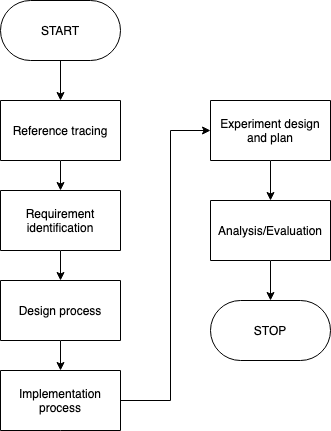
\includegraphics[width=0.7\linewidth]{figure/Metode-Penelitian-flow.png}
	\caption[Metode Penelitian]{}
	\label{fig:metode-penelitian-flow}
\end{figure}


%a. Study Literature
%In this step, this thesis studies the theories needed to design Early Warning System from textbooks, journals, conference papers, thesis or dissertation books, and interview with tea researcher. In this stage, design thinking is also done to  nd out the problems and what are the user needs.
%b. Requirements Analysis
%n this stage, requirements analysis is carried out in accordance with the requirements of the system to be built included requirements of hardware and software (determine tools, materials, and speci cation).
%c. System Design
%A System design and manufacturing device will be done in this stage. System will be designed generally from physical layer to application layer. Arti cial Intelligence algorithm will be implement in this stage too.
%d. testing
%e. Evaluation
%Improve the system according to the feedback that has been obtained. The purpose of this stage is to create a system that is in accordance with user needs.
% f. Final Test, Result and Analysis
%Implementation and testing of the Early Warning and Monitoring System. In this stage, system performance analysis will be carried out.
%g. Reporting
%Writing the  nal report of research and journal publications.

\subsection{Studi Literatur}
Studi literatur tentang :
navigation mobile robot, Behavior based Robotic,  Reinforcement Learning, 
Q-learning, metode Simulasi Mobil Robot dari penelitain sebelumnya.
seperti pada jurnal, karya tulis, serta buku-buku dan literatur referensi yang berkaitan dengan penelitain.

\subsection{Requirement identification}

Pada tahap ini dilakukan analisis yang mencangkup kebutuhan untuk melakukan penelitian, 
kebutuhan yang dianalisis dibagi menjadi analisa data dan juga analisa kebutuhan sistem. 
Analisis dilakukan agar sistem yang dibangun dapat berjalan sesuai dengan rancangan yang sebelumya sudah ditentukan.

\subsection{Perancangan dan Pembuatan Sistem}
Melakukan desain robot dari perangkat lunak dan perangkat keras setelah mempelajari studi literatur dan state of the art
sistem navigasi mobile robot. serta membuat struktur algoritma reinforcement learning, 
berdasarkan pada permasalahan topik penelitian, serta melakukan simulasi pada sistem 
yang dirancang.

\subsection{Implementasi dan Pengujian Sistem}
Melakukan implementasi dan pengujian pada sistem perangkat keras,
pelatihan algoritma reinforcement learning yang digunakan, 
dan menguji perangkat lunak yang telah dirancang, lalu mengevaluasi sistem
berdasarkan topik Penelitian.


\subsection{Pengambilan Data dan Analisa Sistem}
proses pengambilan data dan hasil sesuai dengan tujuan penelitain,
analisa sistem dari hasil dari pengujian sistem.
\subsection{Kesimpulan dan Saran}

\section{Schedule}

%The schedule match the research method and feasible to be realized
%Timetable/Schedule (jadwal pelaksanaan)
%Activity	1	2	3	4	5	..	..
%Reference tracing							
%Requirement identification							
%Design process							
%Implementation process							
%Experiment design and plan							
%Analysis/Evaluation							

Penelitian ini direncanakan akan diselesaikan dalam tempo empat bulan. Rencana tersebut dijabarkan dalam tabel sebagai berikut:

%Pembuatan Usulan Penelitian

%Kajian Pustaka

%Desain algoritma kontrol

%Simulasi Robot

%Pengujian pada robot aktual

%Pembuatan laporan

%Seminar Hasil

\begin{figure}[H]
	\centering
	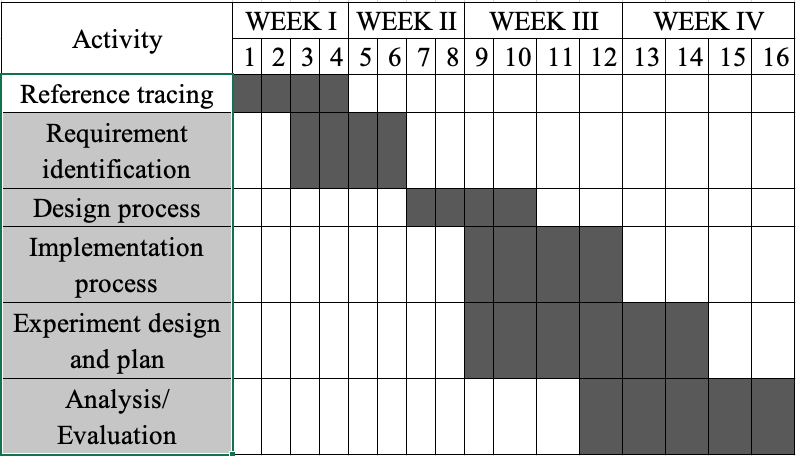
\includegraphics[width=0.9\linewidth]{figure/Chart-ThesisQ.png}
	\caption{Usulan Penelitian}
	\label{fig:chart-thesisq}
\end{figure}





%Contributions
%This thesis has accomplished the proposed goal which is the development of a robot control architecture for an AUV able to achieve simple tasks and exhibit real-time learning capabilities. In the development of this goal, some research contributions were achieved. Hereafter these contributions are listed:

%Online learning of robot behaviors . The most important contribution has been the online learning of robot behaviors. The use of Reinforce- ment Learning in robotics is very common nowadays. However, there are not many approaches which perform an online learning. It is, there- fore, an important contribution to demonstrate the feasibility of the SONQL in a real-time task, specially in a complex domain such as un- derwater robotics. The algorithm proved able to learn the state/action mapping of one DOF in less than 400 iterations, which was less than two minutes. Although the best parameters were used and the exper- iments were designed in detail, these results point out the important role learning algorithms will have in future robotics applications.

%SONQL as a continuous state RL algorithm . The second contribu- tion is also related to the SONQL algorithm. This algorithm demon- strated a high generalization capability in the ”mountain-car” bench- mark. The combination of the Neural Network and the learning sam- ples database resulted in an algorithm able to face the generalization problem. The Neural Network offered a high function approximation capability, and the database guaranteed its stability by avoiding the interference problem. To the best of the author’s knowledge, similar approaches have not been found in the literature and, therefore, the SONQL represents a contribution in the Reinforcement Learning field. However, it must be noted that, although the action space is contin- uous in the Neural Network, the search of greedy actions requires a discretization of this space. Therefore, the SONQL must be considered only as an algorithm to solve the generalization problem in the state space.

%Methodologies for Generalizing . The generalization problem in Rein- forcement Learning was treated in detail. The most important method- ologies currently being applied were described. This study was not considered as an exhaustive survey but a general overview of the most used techniques.

%Development of a behavior-based control system . Another contri- bution was the development of the behavior-based control layer, and in particular, the hybrid coordination methodology. The main features of the coordination system are its simplicity and robustness which assure the safety of the vehicle. In addition, the cooperation between behaviors improves the final robot trajectory. The behavior-based control layer demonstrated as being an efficient tool in the implementation of a set of behaviors and the obtained results were highly satisfactorily.

%Behavior-based control architectures . Four classic Behavior-based con- trol architectures were presented, tested and compared. These archi- tectures represent the most important principles in this field. There- fore, this study offers an exemplified introduction to Behavior-based Robotics. The testing of the architectures in a simulated environment also led to the identification of the dynamics model of ATCR robots.

%tdk d pakai.  ///  jd bahan paper?
%Development of a localization system . A localization system for un- derwater robots in structured environments was proposed. The system is able to estimate the position and orientation in three degrees of free- dom and also the velocity. The localization is based on a coded pattern and a computer vision system. The high accuracy of the estimations and the real-time execution of the algorithm are the main features. The localization system has been one of the most important factors for the success of the presented experiments.